%----------------------------------------------------------------------------
\chapter{Background} \label{background}
%----------------------------------------------------------------------------
%TODO general chapter intro
This chapter provides the necessary theoretical background of the thesis. First, we introduce Model-Based Engineering, then discuss the Foundations of Automata Theory and Automata learning, finally we elaborate upon Specifying Requirements.
%----------------------------------------------------------------------------
\section{Model-Based Engineering} \label{sec_backgrmbe}
%----------------------------------------------------------------------------
Due to the application of the modeling concept in several completely different domains, first of all, we need to define the meaning of \textit{model} in this work.
\begin{definition}[Model]
	A model is the simplified image of an element of the real or a hypothetical world (the system), that replaces the the system in certain considerations.
\end{definition}

For a model to be interpretable, executable or formally verifiable, it must be described according to predefined rules in the given domain. This set of rules is provided by \textit{modeling languages}.
\begin{definition}[Modeling Language]
	A modeling language consists of the following elements:
	\begin{itemize}
		\item \emph{Metamodel:} a model defining the building blocks of the modeling language as well
		as their relationships.
		\item \emph{Concrete syntax:} a set of rules defining a graphical or textual notation for the
		element and connection types defined in the metamodel.
		\item \emph{Well-formedness constraints:} a set of constraints that models have to meet in order
		to be deemed valid in the modeling language.
		\item \emph{Semantics:} a set of rules that define the meaning of the element and connection
		types defined in the metamodel. Semantics can be either \textit{operational} (what should happen during execution) or \textit{denotational} (given by translating concepts in a modeling language to another modeling language with well-defined semantics).
	\end{itemize}
\end{definition}

Models can grasp various aspects of a system. Structural models describe the structure of the system, representing knowledge regarding the parts of the system and the properties and connections of these parts. This means that the model describes static knowledge and not temporal change. On the other hand, behavioral models describe the change of the system over time through its changing of states and execution of processes. These categories do not cover every aspect of a system, and usually cannot be separated this well in practical applications. For instance, action languages of state-based models describe the behavior of the system in a procedural way. There are several possible formalisms for both kinds of models, some of which are discussed in Section \ref{sec_backgrmodeling}.

The process of deriving design artifacts is called \textit{model transformation}.
\begin{definition}[Model Transformation]
	Model transformation is the process of generating the target model from the source model. This process is described by by a transformation definition consisting of transformation rules, and a transformation tool that executes them. A transformation rule is the mapping of elements of the source model to the elements of the target model. \cite{ModelTransformation}
\end{definition}

Model transformations can be categorized based on the types of the source and target models: model-to-model (M2M), model-to-text (M2T), text-to-model (T2M) and text-to-text (T2T). These categories fundamentally define the tools required and usable for handling the different models.

There are also two important factors to consider when designing a model transformation: 
\begin{itemize}
	\item \textit{Consistency}: the same structure or behavior is described by the source and the target models (in their respective domains).
	\item \textit{Traceability}: the images of the original elements of the source model can be traced back to the original elements, from which they were generated.
\end{itemize}

\textbf{Model-Based Systems Engineering (MBSE)} is the formalized application of modeling to support system requirements, design, analysis, verification and validation activities beginning in the conceptual design phase and continuing throughout development and later life cycle phases \cite{mbse}. This concept can also be applied to software engineering. Note, that the models may be the primary artifact of the development process, in which case precisely defined formal models are required. In case the models are the primary artifacts, the process is called \textit{Model-Driven Engineering}.

%----------------------------------------------------------------------------
\section{Foundations of Automata Theory} \label{sec_backgrmodeling}
%----------------------------------------------------------------------------
%TODO DFA, NFA

%TODO LTS (Kripke?)

%TODO Mealy

%TODO Regular languages vs automata

%TODO Omega-regular languages if needed

%TODO Logics (esp LTL) -> ezt külön kiszedjük vagy ide be?

In order to provide the theoretical background of behavioral modeling, this section discusses the necessary basics of formal language and automaton theory.


First, we introduce the fundamentals of formal language theory, on which automaton theory is based on. 

\subsection{Fundamentals of Formal Language Theory}
Atomic elements of formal languages are alphabets, characters and words.

\begin{definition}[Alphabet]
	Let $\Sigma$ be a finite, non-empty set. $\Sigma$ is an alphabet, its elements are symbols or characters.
\end{definition}

\begin{definition}[Word]
	If $\Sigma$ is an alphabet, then any finite sequence comprised of the symbols of $\Sigma$ are words (or Strings). $\Sigma^{n}$ represents the set of every $n$ length word consisting of symbols in $\Sigma$: $\Sigma^{n}: w_1w_2\ldots w_n$, where $\forall 0 \leq i \leq n: w_i \in \Sigma$. The set of every word under an alphabet, formally $\bigcup\limits_{n>0}^{} \Sigma^{n}$ is denoted by $\Sigma^{*}$. The empty word is denoted by $\epsilon$.
\end{definition}

Words can be constructed using other words. The following definition defines these relations.

\begin{definition}[Prefixes, Substrings and Suffixes]
	Let an arbitrary $w = uvs$, where $w, u, v, s\in\Sigma^*$. $u$ is the prefix, $v$ is the substring, and $s$ is the suffix of $w$. Formally:
	\begin{itemize}
		\item $w\in\Sigma^*$ is a prefix of $u\in\Sigma^*$ iff $\exists s\in\Sigma^*: s=wu$,
		\item $w\in\Sigma^*$ is a suffix of $u\in\Sigma^*$ iff $\exists s\in\Sigma^*: s=uw$,
		\item $w\in\Sigma^*$ is a substring of $u, v\in\Sigma^*$ iff $u$ is the prefix and $v$ is the suffix of $w$.
	\end{itemize}
\end{definition}

Using these atomic elements of formal language theory, formal languages can be defined.

\begin{definition}[Formal Language]
	An arbitrary set of words under an Alphabet $\Sigma$ is a Language. Formally: $L\subseteq\Sigma^{*}$.
\end{definition}

\begin{definition}[Prefix-closure]
	Let $L\subseteq\Sigma^*$ and $L' = \{u\in\Sigma^*, v\in\Sigma^* : uv\in L\}$. In other words, L' is the set containing all the prefixes of every word of L. L is prefix-closed if $L = L'$.
\end{definition}

Formal language theory is closely linked with automata theory, which we will introduce in the following subsection.

\subsection{Properties of Deterministic Automata}

Informally, automata are mathematical constructs which read characters from an input and classify them into "accepted" and "rejected" categories. A bit more precisely, automata consist of states, one of which is always active. Starting from an initial state, based on the inputs received, the automaton changes, transitions between states. Essentially, for each of the inputs, the automaton determines whether to keep, or change its current state. In order to determine if an input sequence should be accepted or not, some states are distinguished, accepting states. If after processing a sequence of inputs, the final state of the automaton is an accepting state, the input sequence is accepted. If not, the input is rejected.


One of the most simple automata is the Deterministic Finite Automaton.

\begin{definition}[Deterministic Finite Automaton]
	A Deterministic Finite Automaton is a Tuple of $ DFA=(S,s_{0},\Sigma,\delta,F) $, where: 
	\begin{itemize}
		\item S is a finite, non-epty set containing the states of the automaton,
		\item $s_{0} \in S$ is the initial state,
		\item $\Sigma$ is a finite Alphabet,
		\item $\delta: S\times \Sigma \to S$ is a transition function,
		\item $F\subseteq S$ is a set of the accepting states of the automaton. 
	\end{itemize}
\end{definition}

The deterministic in the name refers to a property of every state having exactly one transition for every input. In other words, every state must have every member of $\Sigma$ listed in its transitions, meaning every state behaves deterministically for every possible input.

An example of a DFA (Deterministic Finite Automaton) from\cite{Steffen2011} can be seen in Example \ref{ex:dfaexample}.

\begin{example}
	\label{ex:dfaexample}
	See Figure \ref{fig:dfaexample}. This example has four states, $S = \{q_0, q_1, q_2, q_3\}$ (hence $|S| = 4$). The initial state is marked by the start arrow, so $s_0 = q_0$. The alphabet can be inferred as $\Sigma = \{a, b\}$. Transitions are visualized as $q_0$ $\xrightarrow[]{\text{a}}$ $q_1$ given by the transition function (in this example) $\delta(q_0, a) = q_1$. The complete transition function in a table form can be seen in Table \ref{tab:dfaexampledelta}. Finally, the accepting states, or in this case, accepting state of the automaton is $F = \{q_3\}$.
\end{example}


The semantics of automata are defined via runs. A run of an automaton is to test for a certain input (word), if it is accepted or rejected. See Example \ref{ex:dfaruns}.

\begin{example}
	\label{ex:dfaruns}
	In accordance with the transition function, a run of Figure \ref{fig:dfaexample} with an input of $\{a, a, a\}$ would end in state $q_3$ meaning the input is accepted. A rejected input could be $\{a, b, b\}$, which would stop at state $q_1$, a non-accepting state. On deeper examination, one can see, that this automaton only accepts runs with inputs containing $4i+3 a$.
\end{example}

\begin{figure}[!ht]
	\centering
	\begin{tikzpicture}[shorten >=1pt,node distance=3cm,on grid,auto] 
	\node[state,initial] (q_0)   {$q_0$}; 
	\node[state] (q_1) [right=of q_0] {$q_1$}; 
	\node[state] (q_2) [below=of q_0] {$q_2$}; 
	\node[state,accepting](q_3) [right=of q_2] {$q_3$};
	\path[->] 
	(q_0) edge  node {a} (q_1)
	edge [loop below] node {b} ()
	(q_1) edge  node[pos=0.62]  {a} (q_2)
	edge [loop below] node {b} ()
	(q_2) edge  node [swap] {a} (q_3) 
	edge [loop above] node {b} ()
	(q_3) edge  node[pos=0.62] [swap] {a} (q_0)
	edge [loop above] node {b} () ;
	\end{tikzpicture}
	\caption{A simple DFA from \cite{10.1007/978-3-319-11164-3_26}.}
	\label{fig:dfaexample}
\end{figure}

\begin{table}[!ht]
	\centering
	\begin{tabular}{|c|cccc|}
		\hline
		$\delta$ & $q_0$ & $q_1$ & $q_2$ & $q_3$\\ \cline{1-5}
		a & $q_1$ & $q_2$ & $q_3$ & $q_0$ \\	
		b & $q_0$ & $q_1$ & $q_2$ & $q_3$ \\	\hline
	\end{tabular}
	\caption{The transition function of the automaton seen in Figure \ref{fig:dfaexample}}
	\label{tab:dfaexampledelta}
\end{table}

A slightly different formalism can be defined for cases where the acceptance of the input (word) is not necessary to consider, called Labeled Transition System.

\begin{definition}[Labeled Transition System]
	A Labeled Transition System is a Tuple $LTS=(S, Act, \rightarrow)$, where:
	\begin{itemize}
		\item $S={q_0, q_1, ..., q_n}$ the finite, non-empty set of states, $q_0$ being the initial state,
		\item $Act = {a, b, c, ...}$ the finite set of actions,
		\item $\rightarrow \subseteq S \times Act \times S$ the labeled transitions between the states.
	\end{itemize}
	In the beginning, the initial state is active. The active state may change after each transition.
	
	The \textit{path} of an LTS is the $\pi = (q_0, a_1, q_1, a_2, ...)$ alternating sequence of states and actions, where $q_0$ is the initial state and the subsequent states are the results of the transitions labeled with the actions of the same index. 
\end{definition}

\begin{example}
	\label{ex:ltsexample}
	See Figure \ref{fig:ltsexample}. This example has three states, $S = \{q_0, q_1, q_2\}$ (hence $|S| = 3$). The initial state is $q_0$, also marked by the start arrow. The set of actions is $Act = \{money, coffee, tea\}$. Transitions are visualized as $q_0$ $\xrightarrow[]{\text{money}}$ $q_1$ given by the transition (in this example) $(q_0, money, q_1)$. The set of transitions ($\rightarrow$) also contains $(q_1, coffee, q_2)$ and $(q_1, tea, q_3)$.
\end{example}

\begin{figure}[!ht]
	\centering
	\begin{tikzpicture}[shorten >=1pt,node distance=3cm,on grid,auto] 
		\node[state, initial] (s_1)   {$q_0$}; 
		\node[state] (s_2) [below=of s_1] {$q_1$}; 
		\node[state] (s_3) [left=of s_2] {$q_2$}; 
		\node[state](s_4) [right=of s_2] {$q_3$};
		\path[->] 
		(s_1) edge  node {money} (s_2)
		(s_2) edge  node[pos=0.62]  {coffee} (s_3)
		(s_2) edge  node [swap] {tea} (s_4) ;
	\end{tikzpicture}
	\caption{A simple LTS}
	\label{fig:ltsexample}
\end{figure}

DFAs and LTSs are useful to model system behavior based on inputs, but in order to work with reactive systems, we also need to handle outputs. Mealy machines are automata designed to communicate with output symbols instead of accepting and rejecting states.


\begin{definition}[Mealy machine]
	A Mealy machine or Mealy automaton is a Tuple of $ M=(S,s_{0},\Sigma,\Omega,\delta,\lambda) $, where:
	\begin{itemize}
		\item S is a finite, non-empty set containing the states of the automaton,
		\item $s_{0} \in S$ is the initial state,
		\item $\Sigma$ is the input alphabet of the automaton,
		\item $\Omega$ is the output alphabet of the automaton,
		\item $\delta: Q\times \Sigma \to Q$ is the transition function and
		\item $\lambda: Q\times \Sigma \to \Omega$ is the output function. 
	\end{itemize}
\end{definition}

Mealy machines can be regarded as deterministic finite automata over the union of the input alphabet and an output alphabet with just one rejection state, which is a sink, or more elegantly, with a partially defined transition relation.\cite{Steffen2011}

An example of a deterministic Mealy machine can be seen in Example \ref{ex:coffeemealy}.

\begin{example}
	\label{ex:coffeemealy}
	An example of a deterministic Mealy machine can be seen in Figure \ref{fig:coffeemealy}. The formal definition of the automaton can be seen below.
	\begin{itemize} 
		\item $S = \{a, b, c, d, d', e, f\}$ 
		\item $s_0 = a$
		\item $\Sigma = \{water, pod, button, clean\}$
		\item $\Omega$ = \{$\checkmark$, \Coffeecup, $\star$\}
	\end{itemize}
	The transitions, as seen in Figure \ref{fig:coffeemealy} are visualized as $s_0$ $\xrightarrow[]{\text{input/output}}$ $s_1$, which denotes the machine moving from state $s_0$ to state $s_1$ on the specified input, while causing the specified output. Also, some simplifications are done, e.g. in this transition: d $\xrightarrow[]{\text{\{water,pod\}/\checkmark}}$ d we see a visual simplification of having both transitions merged to one arrow, this is only for visual convenience. Figure \ref{fig:coffeemealy} is also a great example of sinks, as seen in state f, the machine accepts anything, and never changes. This is a variation of the accepting state seen in DFAs.
\end{example}

\begin{figure}[!ht]
	\centering
	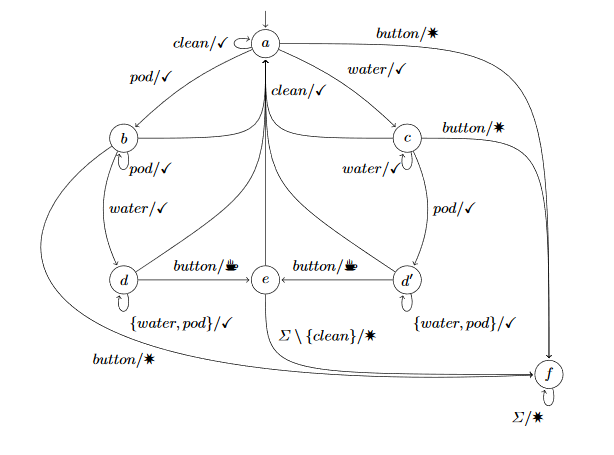
\includegraphics[width=0.7\linewidth]{figures/coffeemealy}
	\caption{Mealy machine representing the functionality of a coffee machine.\cite{Steffen2011}}
	\label{fig:coffeemealy}
\end{figure}

Since automaton-based formalisms deal with alphabets, formal language theory is essential not only to define them, but to construct them in a way that is efficient in practical applications. Often automata are used to design and analyze real-life systems. Naturally, questions of efficiency and correctness arise, which is why the relations of automatons and formal languages are discussed more in-depth in the following subsection.

\subsection{Relations of Formal Languages and Automata}

\begin{definition}[Recognized language of automata]
	The language $L\subseteq\Sigma$ containing all the accepted words by an automaton M is called the recognized language of the automaton. It is denoted by L(M) = L.
\end{definition}

\begin{definition}[Regular language]
	A formal language L is regular, iff there is a Deterministic Finite Automaton M, for which L(M) = L, in other words, iff there is a DFA with the recognized language of L.
\end{definition}

Let us now introduce a semantic helper $\delta^*$ for both DFAs and Mealy machines. $\delta^*$ is an extension of the $\delta$ transition function, as $\delta^*: S\times\Sigma^* \to S$ defined by $\delta^*(s,\epsilon) = s$ and $\delta^*(s, \alpha w) = \delta^*(\delta(s, \alpha), w)$, essentially providing the state of the automaton after running an input sequence from a specified state.

\begin{definition}[Myhill-Nerode relation] 
	A DFA $M=(S,s_{0},\Sigma,\delta,F)$ induces the following equivalence relation $\equiv_M$ on $\Sigma^*$ (when L(M) = $\Sigma$):\\
	\null\qquad$x\equiv_M y \iff \delta^*(s, x) = \delta^*(s, y)$\\
	where $x, y\in\Sigma^*$. This means, that x and y are equivalent with respect to $\equiv_M$.\cite{Kozen1977}.
\end{definition}

In words, the Myhill-Nerode relation states, that two words are equivalent wrt. $\equiv_M$ iff runs of both words would end in the same state on the automaton M. The Myhill-Nerode relation is an equivalence relation with some additional properties\cite{Kozen1977}, which can be seen in the following.


\begin{itemize}
	\item The properties of equivalence relations:
	\begin{itemize}
		\item Reflexivity: $x\equiv_M x$.
		\item Symmetry: $x\equiv_M y \implies y\equiv_M x$.
		\item Transitivity: if $(x\equiv_M y$ and $y\equiv_M z) \implies x\equiv_M z$.
	\end{itemize}
	\item Right congruence: $\forall x, y\in\Sigma^*: (x\equiv_M y \implies 		\forall a\in\Sigma: xa\equiv_Mya)$\\ also, by induction, this can be extended to:\\
	$\forall x, y\in\Sigma^*: (x\equiv_M y \implies \forall w\in\Sigma^*: xw\equiv_Myw)$. 
	\item It respects membership wrt. R:\\
	$\forall x, y\in\Sigma^*: x\equiv_M y \implies (x\in R \iff y\in R)$.
	\item $\equiv_M$ is of finite index, has finitely many equivalency classes. Since for every state $s\in S$, the sequences which end up in s are in the same equivalence class, the number of these classes is exactly $|S|$, which is a finite set.
\end{itemize}

Using this relation, we can introduce the Myhill-Nerode theorem, which neatly ties together the previous definitions.

\begin{theorem}[Myhill-Nerode theorem\cite{Kozen1977}\cite{10.2307/2033204}]
	Let $L\subseteq\Sigma^*$. The following three statements are equivalent:
	\begin{itemize}
		\item L is regular.
		\item there exists a Myhill-Nerode relation for L.
		\item the relation $\equiv_L$ is of finite index.
	\end{itemize}
	For proof, see \cite{Kozen1977}\cite{10.2307/2033204}.
\end{theorem}

The same concepts can be applied to Mealy machines, which are somewhat more complex in this regard. As before, a semantic helper is needed similar to $\delta^*$, but considering the output function of Mealy machines. $\lambda^*: S\times\Sigma^* \to \Omega$, defined by $\lambda^*(s, \epsilon) = \varnothing$ and $\lambda^*(s, w\alpha) = \lambda(\delta^*(s, w), \alpha)$.



When monitoring the behavior of Mealy machines, one of the most important metrics given an input is the specific output given by the input. The behavior of a Mealy machine, a specific run of it, has a pattern of \textit{$i_1,o_1,i_2,o_2,..,i_n,o_n$}, where \textit{i} are inputs and \textit{o} are outputs. In order to characterize these runs, we actually do not need every output from this pattern, we only need the final one. Also note, that essentially the final output of a run is given by $\lambda^*(s_0, inputs)$. Let us introduce a $\llbracket M\rrbracket$: $\Sigma^*\to\Omega$ semantic functional as  $\llbracket M\rrbracket(w) = \lambda^*(s_0, w)$. This provides the final output given by a run of an automaton for an input sequence $w$. Using $\llbracket M\rrbracket$, the behavior of Mealy machines can be captured, as discussed in the following.

\begin{example}
	Given the Mealy machine $M\textsubscript{coffeemachine}$ in Figure \ref{fig:coffeemealy}, the runs:\\
	\null\qquad<clean, $\checkmark$>, \\
	\null\qquad<pod water button, \Coffeecup> \\
	are in $\llbracket M\textsubscript{coffeemachine}\rrbracket$, since the given input words cause the corresponding outputs, while the runs\\
	\null\qquad<clean, \Coffeecup> and \\
	\null\qquad<water button button, $\checkmark$> \\
	are not, since these input sequences do not produce those outputs.
\end{example}

Similarly to the Myhill-Nerode relations in DFAs, equivalence relations over the $P: \Sigma^*\to\Omega$ functional can be introduced, where P is an abstraction of  $\llbracket M\rrbracket$ that can be applied to any state, rather than just the initial state.

\begin{definition}[Equivalence of words wrt. $\equiv_P$\cite{Steffen2011}]
	Given a Mealy machine $M=(S,s_{0},\Sigma,\Omega,\delta,\lambda) $, two words, $u, u'\in\Sigma^*$ are equivalent with respect to $\equiv_P$:\\
	$u \equiv_P u' \iff (\forall v\in\Sigma^*:P(s, uv) = P(s, u'v))$.\\
	We write [u] to denote the equivalence class of u wrt. $\equiv_P$.
\end{definition}

This definition is more along the lines of the right congruence property observed in the Myhill-Nerode relations. The original formalism: $u \equiv_P u' \iff P(s, u) = P(s, u')$ of the Myhill-Nerode relation still stands as a special case of the above definition: if $v=\epsilon$ and $v'=\epsilon$, $P(s, uv) = P(s, u)$ and $P(s, u'v) = P(s, u')$.

\begin{example}
	Taking Figure \ref{fig:coffeemealy} as an example, the following words are equivalent wrt. $\equiv_{\llbracket M\rrbracket}$:\\
	\null\qquad\qquad\qquad\qquad\space $water, pod$\\
	\null\qquad\qquad$\equiv_{\llbracket M\rrbracket}$\qquad $water, water, pod$\\
	\null\qquad\qquad$\equiv_{\llbracket M\rrbracket}$\qquad $pod, pod, water$.
	
	The first two of $\equiv_{\llbracket M\rrbracket}$ are straightforward, since both words lead to the same state, $d'$, while the third input ends in state $d$. Observably, state $d$ and $d'$ wrt. outputs operate exactly the same regardless of continuation, hence the equivalence holds.
\end{example}

\begin{theorem}[Characterization theorem\cite{Steffen2011}]
	Iff mapping $P: \Sigma^*\to\Omega$ $\equiv_P$ has finitely many equivalence classes, there exists a Mealy machine M, for which P is a semantic functional.
	\\\\
	\textit{Proof}($\impliedby$): As seen in the case of the Myhill-Nerode finite index property for DFAs, same states in Mealy machines will obviously be in same equivalence classes. This implies, that the number of classes in (or in other words, the index of) $\equiv_P$ is at most the number of states the Mealy machine contains, which is finite by definition.
	\\
	\textit{Proof}($\implies$): Consider the following Mealy machine: $M_P=(S,s_{0},\Sigma,\Omega,\delta,\lambda)$:\\
	\null\qquad -S is given by the equivalence classes of $\equiv_P$.\\
	\null\qquad -$s_0$ is given by $[\epsilon]$.\\
	\null\qquad -$\delta$ is defined by $\delta([u], \alpha) = [u\alpha]$.\\
	\null\qquad -$\lambda$ is defined by $\lambda([u], \alpha) = o$, where $P(u\alpha) = o$.\\
	A Mealy machine constructed this way fulfills what the theorem states, P is a semantic functional of it, in other words, $\llbracket M\rrbracket$ = P.
\end{theorem}

With this theorem, regularity for mappings $P:\Sigma^*\to\Omega$ can be defined. A $P:\Sigma^*\to\Omega$ mapping is regular, iff there is a corresponding Mealy machine for which $\llbracket M\rrbracket$ = P, or equivalently, if P has a finite number of equivalence classes, analogously to the previously seen "classical" regularity.

\subsection{Minimization of Automata}

The introduction of regularity is useful in the construction of automata, specifically, the construction of canonical automata. 


\begin{figure}
	\centering
	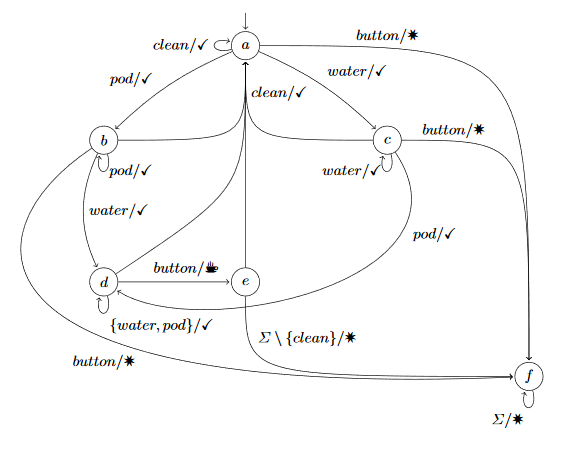
\includegraphics[width=0.7\linewidth]{figures/coffeemealyminimal}
	\caption{Minimal version of the Mealy machine seen in \ref{fig:coffeemealy}}
	\label{fig:coffeemealyminimal}
\end{figure}


\begin{definition}[Canonical automaton (Minimal automaton)]
	An automaton M is canonical (i.e. minimal) iff:
	\begin{itemize}
		\item every state is reachable: $\forall s\in S: \exists w\in\Sigma^*: \delta^*(s_0, w) = s$,
		\item all states are pairwisely separable, in other words behaviorally distinguishable. For Mealy machines, this is formalized as: $\forall s_1, s_2\in S: \exists w\in\Sigma^*: \lambda(s_1, w)\neq\lambda(s_2, w)$
	\end{itemize}
\end{definition}

The minimal version of the Mealy machine in Figure \ref{fig:coffeemealy} can be seen in Figure \ref{fig:coffeemealyminimal}.


Constructing automata to be canonical, especially in the case of Mealy machines is important with regards to efficiency and is the backbone of automaton learning. The next proposition comes straightforward from the previously presented characterization theorem.


\noindent \textbf{Proposition (Bounded reachability\cite{Steffen2011})}: Every state of a minimal Mealy machine with n states has an access sequence, i.e., a path from the initial state to the given state,  of  length  at  most n-1.  Every  transition  of the model can be covered by a sequence of length at most n from the initial state.

The process of constructing automata uses the concept of partition refinement. It works based on distinguishing suffixes, suffixes of words which mark, witness the difference between two access sequences. The following notion is introduced to formalize this.


\begin{definition}[k-distinguishability\cite{Steffen2011}]
	Two states, $s,s'\in S$ are k-distinguishable iff there is a word $w\in\Sigma^*$ of length k or shorter, for which $\lambda^*(s, w)\neq\lambda^*(s',w)$.
\end{definition} 

\begin{definition}[exact k-distinguishability]
	Two states, $s,s'\in S$ are exact k-distinguishable, denoted by $k^=$ iff s and s' are k-distinguishable, but not (k-1)-distinguishable
\end{definition}

Essentially, if two states, s and s' are  k-distinguishable, then when processing the same input sequence, from some suffix of the word w with length at most k, they will produce differing outputs. Using this, we can observe, that whenever two states, $s_1, s_2\in S$ are (k+1)-distinguishable, then they each have a successor $s_1'$ and $s_2'$ reached by some $\alpha\in\Sigma$, such that $s_1'$ and $s_2'$ are k-distinguishable. These successors are called $\alpha$-successors. This suggests, that:
\begin{itemize}
	\item no states are 0-distinguishable and
	\item two states $s_1$ and s2 are (k+1)-distinguishable iff there exists an input symbol $\alpha\in\Sigma$, such that $\lambda(s_1, \alpha) \neq \lambda(s_2,\alpha)$ or $\delta(s_1, \alpha)$ and $\delta(s_2, \alpha)$ are k-distinguishable.\cite{Steffen2011}
\end{itemize}
This way, if we have an automaton M, we can construct its minimal version, by iteratively computing k-distinguishability for increasing k, until stability, that is until the set of exactly k-distinguishable states is empty.

\begin{example}
	Given the Mealy machine seen in Figure \ref{fig:coffeemealy}, we can use k-distinguishability to refine its partitions. The initial state, the initial partition would be:\\
	$P_1 = \{a, b, c\}, \{d, d'\}, \{e\}, \{f\}$\\
	since when k=1, a, b and c are not 1-distinguishable, but d and d' separate on the behavior of the \textit{button} input, while e and f are separated by the suffix \textit{clean}. Let's see the k=2 scenario.\\
	$P_2 = \{a\}, \{b\}, \{c\}, \{d, d'\}, \{e\}, \{f\}$\\
	Here, \textit{water} and \textit{pod} separate a, b and c, while d and d' can still no longer be separated. If observed, even if k is increased, d and d' can not be refined. This means, that they are indistinguishable, they can be merged together without altering behavior. This shows the process of acquiring the minimal machine seen in Figure \ref{fig:coffeemealyminimal}.
	\label{ex:partitionrefinement}
\end{example} 

The process explained in Example \ref{ex:partitionrefinement} is partition refinement, the exact algorithm and proof of its validity can be seen in \cite{Steffen2011}. Partition refinement is a version of the minimization algorithm for DFAs proposed by Hopcroft\cite{HOPCROFT1971189}. 

Let us define one last relation which will be useful in the next section to compare automata minimization and automata learning.

\begin{definition}[k-epimorphisms]
	Let $M=(S,s_{0},\Sigma,\Omega,\delta,\lambda)$ and $M=(S',s_{0}',\Sigma,\Omega,\delta',\lambda')$ be two Mealy machines with shared alphabets. We call a surjective function $f_k: S \to S'$ existential k-epimorphism between $M$ and $M'$, if for all $s'\in S', s\in S$ where $f_k(s) = s'$ and with any $\alpha\in\Sigma$, we have: $f_k(\delta(s,\alpha)) = \delta'(s',\alpha)$, and all states, that are mapped by $f_k$ to the same state of $M'$ are not k-distinguishable.
\end{definition}

It is straightforward to establish that all intermediate models arising during the partition refinement process are images of the considered Mealy machine under a k-epimorphism, where k is the number of times all transitions have been investigated.\cite{Steffen2011} Essentially this establishes $P_1$ and $P_2$ from Example \ref*{ex:partitionrefinement} as images of the Mealy machine seen in Figure \ref{ex:coffeemealy} under k-epimorphisms where k=1 and k=2 respectively.

Active automaton learning algorithms operate in a similar way, but they do not have access to the automata they are learning.

%----------------------------------------------------------------------------
\section{Automata Learning} \label{sec_backgrautomatalearning}
%----------------------------------------------------------------------------
%TODO active vs passive

%TODO Active

%TODO DHC

\paragraph{Automata Learning}  is a way of modeling a system without having specific knowledge of its internal behavior. To accomplish this, the external behavior of the system needs to be observed. This learned model is, as the name suggests, an automaton. 
\\Formally: Automata  learning is  concerned  with  the  problem  of  inferring  an automaton model for an unknown formal language $L$ over some alphabet $\Sigma$\cite{Howar2018}.
\\\\In order to monitor a system, access to its behavioral information is required. There are two approaches, which separate the two types of automaton learning.

\paragraph{Passive Automata Learning} In case of passive automaton learning, the gathering of information is not part of the learning process, but rather a prerequisite to it. The learning is performed on a pre-gathered positive an/or negative example set of the systems behavior. In passive automaton learning, the success of the process is determined not only by the efficiency of the algorithm, but the methodology and time used to gather the data.

\paragraph{Active Automata Learning} In case of active automaton learning, the behavioral infromation is gathered by the learning algorithm via queries. In order to accomplish this, learning is separated to two components: the learner, which learns, and the teacher, which can answer questions about the system under learning.


Active automaton learning follows the MAT, or the Minimally Adequate Teacher model proposed by Dana Angluin\cite{ANGLUIN198787}. It defines the separation of the algorithm to a teacher and a learner component in a way, where the teacher can only answer the minimally adequate questions needed to learn the system. These two questions, or queries are are follows:


\paragraph{Membership query} Given a $w\in\Sigma^{*}$ word, the query return the $o\in \Omega$ output o corresponding to it, treating the word as a string of inputs. We write $mq(w) = o$ to denote that executing the query w on the system under learning (SUL) leads to the output o: $\llbracket SUL \rrbracket(w) = o$ or $\lambda^*(s_0, w) = o$.

\paragraph{Equivalence query} Given a hypothesis automaton $M$, the query attempts to determine if the hypothesis is behaviorally equivalent to the SUL, and if not, finding the diverging behavior, and return with an example. We write $eq(H) = c$, where $c\in\Sigma^*$, to denote an equivalence query on hypothesis H, returning a counterexample c. The counter example provided is the sequence of inputs for which the output of system under learning and the output of the hypothesis differ: $ \llbracket H\rrbracket(c) \neq mq(c)$.

\noindent The learner component uses membership queries to construct a hypothesis automaton, then refines this hypothesis by the counterexamples provided by equivalence queries. Once counterexamples can not be found this way, the learners hypothesis is behaviorally equivalent to the SUL. The learning can terminate and the output of the learning is the current hypothesis.

%TODO: diagram legyen korrekt uml
\begin{figure}[!ht]
	\centering
	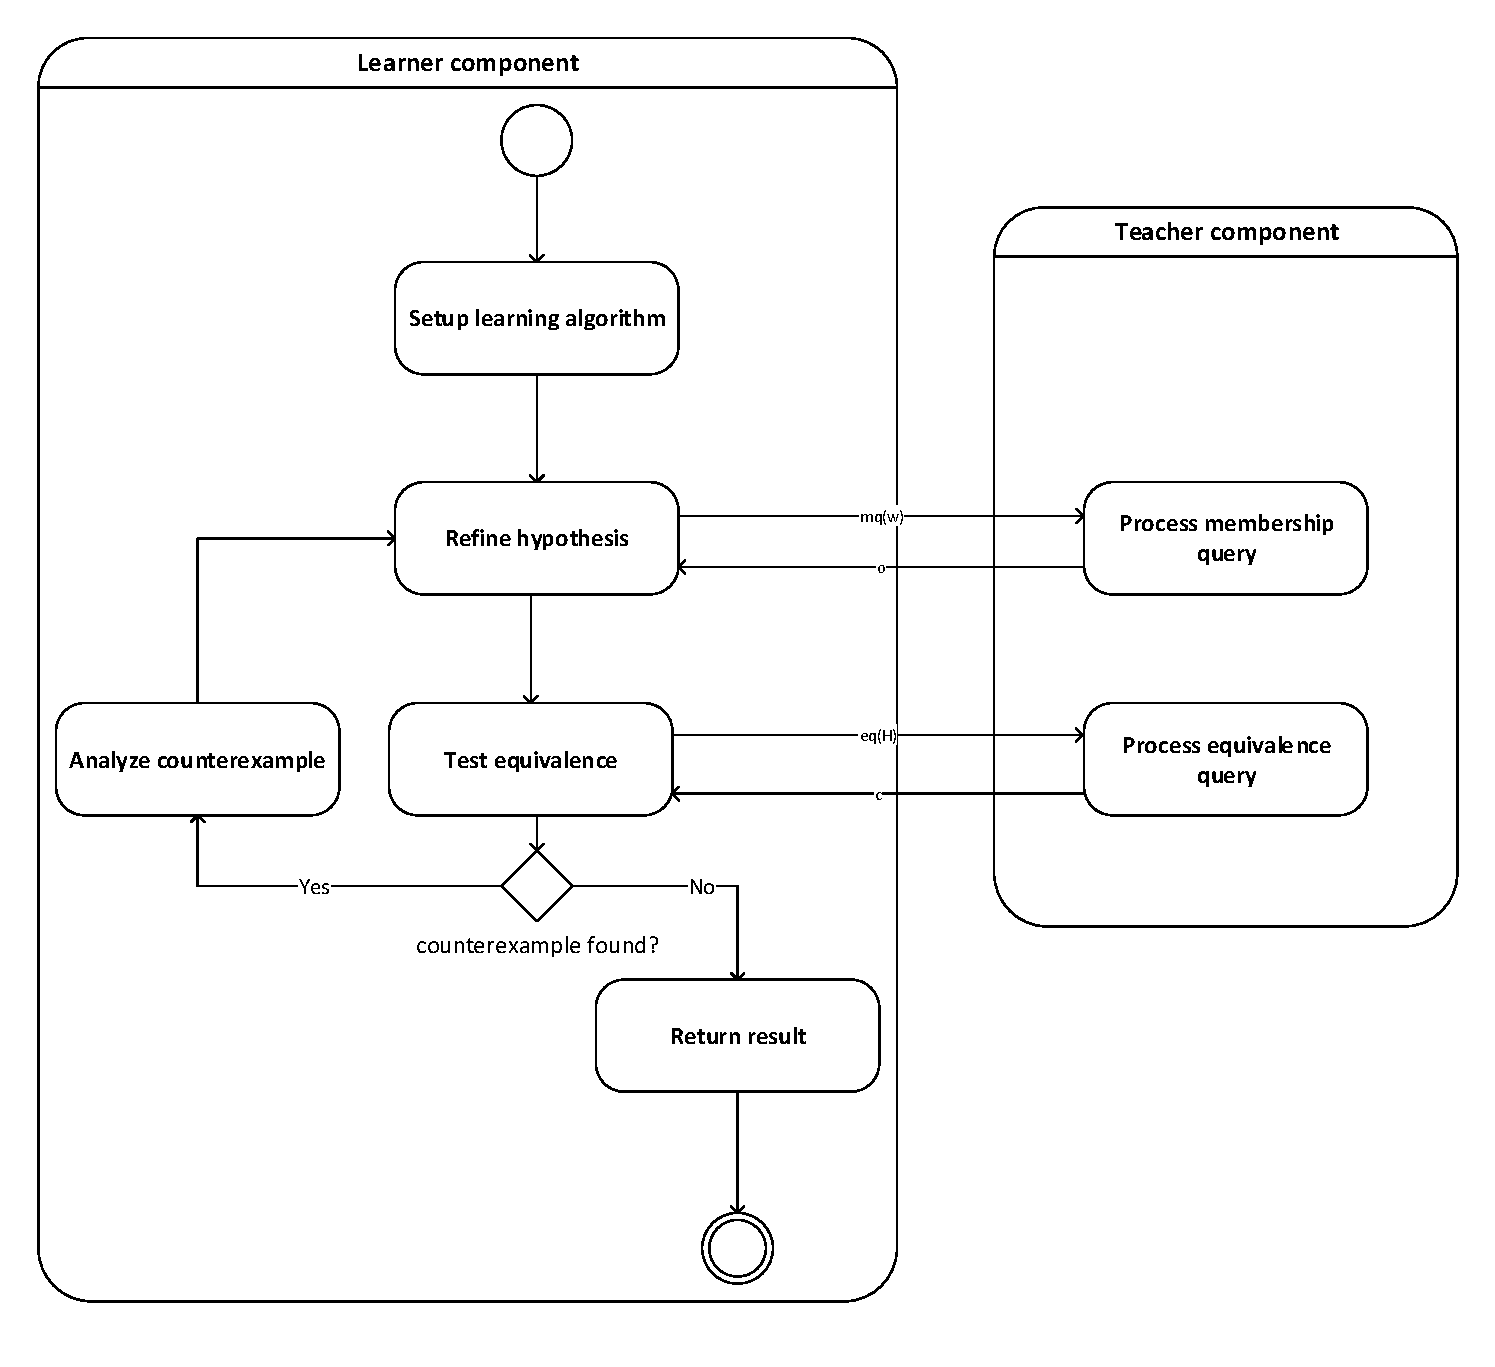
\includegraphics[width=1.0\linewidth]{figures/flowchartlearning}
	\caption{Active automaton learning}
	\label{fig:flowchartlearning}
\end{figure}

As seen on Figure \ref{fig:flowchartlearning}, the learning proceeds in rounds, generating and refining hypothesis models by exploring the SUL via membership queries. As the equivalence checks produce counterexamples, the next round of this hypothesis refinement is driven by the counterexamples produced.

Using an analogous strategy to the minimization of automata seen in the previous section, starting only with a one state hypothesis automaton, all words are explored in the alphabet in order to refine and extend this hypothesis. Here, there is a dual way of characterizing (and distinguishing) between states\cite{Steffen2011}:
\begin{itemize}
	\item By words reaching them. A prefix-closed set $S_p$ of words, reaching each state exactly once, defines a spanning tree of the automaton. This characterization aims at providing exactly one representative element from each class of $\equiv_P$ on the SUL. Active learning algorithms incrementally construct such a set $S_p$. \\This prefix-closedness is necessary for $S_p$ to be a "spanning tree" of the Mealy machine. Extending $S_p$ with all the one-letter continuations of words in $S_p$ will result in the tree covering all the transitions of the Mealy machine. $L_p$ will denote all the one-letter continuations that are not already contained in $S_p$.
	\item By their future behavior with respect to an increasing vector of words of $\Sigma^*$. This vector $<d_1, d_2,...,d_k>$ will be denoted by $D$, and contains the "distinguishing suffixes". The corresponding future behavior of a state, here given in terms of its access sequence $u\in S_p$, is the output vector$<mq(u*d_1), ..., mq(u*d_k)>\in\Omega^k$, which leads to an upper approximation of the classes of $\equiv_{\llbracket SUL\rrbracket}$. Active learning incrementally refines this approximation by extending the vector until the approximation is precise.
\end{itemize}
While the second characterization defines the states of the automaton, where each output vector corresponds to one state, the spanning tree on $L_p$ is used to determine the transitions of these states. In order to characterize the relation between the SUL $M=(S,s_{0},\Sigma,\Omega,\delta,\lambda)$ and the hypothesis model $M'=(S',s_{0}',\Sigma,\Omega,\delta',\lambda')$ (note, that $M$ and $M'$ only share alphabets), the following definition is introduced. 

\begin{definition}[D-epimorphism]
	Let $D\subseteq\Sigma^*$. We call a surjective function $f_D:S\to S'$ existential D-epimorphism (surjective homomorphism) between $M$ and $M'$ if, for all $s'\in S'$ there exists an $s\in S$ with $f_D(s) = s'$ such that for all $\alpha \in \Sigma$ and all $d\in D$: $f_D(\delta(s, \alpha)) = \delta'(s', \alpha)$, and $\lambda^*(s,d) = \lambda^*(s', d)$. 
\end{definition}

Note, that active learning deals with canonical Mealy machines, in other words, the canonical form of SUL, and not, the perhaps much larger Mealy machine of SUL itself. 

Since active learning algorithms maintain an incrementally growing extended spanning tree for $H=(S_H, h_0, \Sigma, \Omega, \delta_H, \lambda_H)$, i.e., a prefix-closed set of words reaching all its states and covering all transitions, it is straightforward to establish that these hypothesis models are images of the canonical version of SUL under a canonical existential D-epimorphism, where D is the set of distinctive futures underlying the hypothesis construction\cite{Steffen2011}
\begin{itemize}
	\item define $f_D : S_{SUL}\to S_H$ by $f_D(s) = h$ as following: if $\exists w\in S_p \cup L_p$, where $\delta(s_0, w) = s$, then $h = \delta_H(h_0,w)$. Otherwise h may be chosen arbitrarily.
	\item It suffices to consider the states reached by words in the spanning tree to establish the defining properties of $f_D$. This straightforwardly yields:
	\begin{itemize}
		\item $f_D(\delta(s,\alpha)) = \delta_H(h, \alpha)$ for all $\alpha\in\Sigma$, which reflects the characterization from below.
		\item $\lambda^*(s, d) = \lambda^*_H(h,d)$ for all $d\in D$, which follows from the maintained characterization from above.\cite{Steffen2011}
	\end{itemize}
\end{itemize}

In basic logic, D-epimorphisms and k-epimorphisms do not differ, they both deal with establishing constructed models being images of the model they are based on. D-epimorphisms could replace k-epimorphisms where $D=\Sigma^k$, it can be suggested, that there is no need to differentiate. However, there is in important difference of complexity between the two. While k-distinguishability supports polynomial time, black-box systems do not. Also, the "existential" in existential D-epimorphism is important: $f_D$ must deal with unknown states, ones that haven't been encountered yet. This implies that characterization can only be valid for already encountered states.

Active learning algorithms can be proven correct using the following three-step pattern:
\begin{itemize}
	\item Invariance: The number of states of each hypothesis has an upper bound of $\equiv_{\llbracket SUL\rrbracket}$.
	\item Progress: Before the final partition is reached, an equivalence query will provide a counterexample, where an input word leads to a different output on the SUL and on the hypothesis. This difference can only be resolved by splitting at least one state, which increases the state count.
	\item Termination: The refinement terminates after at most the index of $\equiv_{\llbracket SUL\rrbracket}$ many steps, caused directly by the described invariance and progress properties.
\end{itemize}

The following subsection introduces the first active automaton learning algorithm this thesis covers.

\subsection{Direct Hypothesis Construction\cite{10.1007/978-3-642-34781-8_19}}
The Direct Hypothesis Construction algorithm, which hypothesis construction can be seen in Algorithm \ref{algo:dhc}  follows the idea of the breath-first search of graph theory. It constructs the hypothesis using a queue of states, which is initialized with the states of the spanning tree to be maintained. Explored states are removed from this queue, while the discovered successors are enqueued, if they are provably new states. The algorithm starts with a one-state hypothesis, including only the initial state, reached by $\epsilon$ and D = $\Sigma$. It then tries to complete the hypothesis: for every state, the algorithm determines the behavior of the state under D. This behavior is called the extended signature of said state. States with a new extended signatures are provably new states, so to guarantee further investigation, all their successors are enqueued. Initially, $D=\Sigma$, so only the $1^=$-distinguishable states are revealed during the first iteration. This is extended straightforwardly to comprise a prefix closed set of access sequences. \cite{Steffen2011}\cite{10.1007/978-3-642-34781-8_19}

\begin{algorithm}[H]
	\SetAlgoLined
	\DontPrintSemicolon
	\KwIn{$S_p$: a set of access sequences, D: a set of suffixes, an input alphabet $\Sigma$}
	\KwOut{A Mealy machine $H=(S, s_0, \Sigma, \Omega, \delta, \lambda)$}
	initialize hypothesis H, create a state for all elements of $S_p$\;
	initialize a queue Q with the states of H\;
	\While{Q is not empty}{
		s = dequeue state from Q\;
		u = access sequence from $s_0$ to s\;
		\For{$d\in D$}{
			o = mq($u\*d$)\;
			set $\lambda(s,d) = o$\;
		}
		\eIf{exists an $s'\in S$, where the output signature of $s'$ is the same as $s$}{
			reroute transitions of $s$ to $s'$ in H\;
			remove $s$ from H\;
		}{
			create and enqueue successors of $s$ for every input in $\Sigma$ into Q, if not already in $S_p$\;
		}
	}
	Remove entries of $D\setminus\Sigma$ from $\lambda$\;
	\Return{H}\;
	\caption{Hypothesis construction of the Direct Hypothesis Construction algorithm as seen in \cite{Steffen2011}.}
	\label{algo:dhc}
\end{algorithm}

After the execution of the Hypothesis construction seen in Algorithm \ref{algo:dhc}, the output automaton H is used in an equivalence query $eq(H) = c$, to find if a counterexample $c$ exists. If no counteraxamle can be found, the learning terminates, $H$ is the learned automaton. Else, if a counterexample $c$ is found, for which $\lambda_H(s_0,c) \neq mq(c)$, $c$ is used to enlarge the suffixes in D and a new iteration of Algorithm \ref{algo:dhc} begins, using the now extended set D and all the access sequences found in the previous iteration (the current spanning tree $S_p$).

The DHC algorithm is a straightforward implementation of active automata learning. It terminates after at most $n^3mk+n^2k^2$ membership queries, and $n$ equivalence queries, where $n$ is the number of states in the final hypothesis, $k$ is the longest set of inputs, and $m$ is the length of the longest counterexample\cite{10.1007/978-3-642-34781-8_19}.

\clearpage
%----------------------------------------------------------------------------
\section{Specifying Requirements} \label{sec_backgrspecreq}
%----------------------------------------------------------------------------

The previous sections introduced different modeling types and techniques. We now discuss the requirements used in model-based engineering which the models need to satisfy.

%----------------------------------------------------------------------------
\subsection{Requirements} \label{subs_backgrreq}
%----------------------------------------------------------------------------

Throughout this thesis, the concept of requirements is going to be used widely, therefore, it is essential to define it precisely. 

\begin{definition}[Requirement\cite{sweterminology}]
	\mbox{}
	\begin{enumerate}
		\setlength\itemsep{0.1em}
		\item A condition or capability needed by the user to solve a problem or achieve an objective.
		\item A condition or capability that must be met or possessed by a system component to satisfy a contract, standard, specification or other formally imposed documents.
		\item A documented representation of a condition or capability as in (1) or (2).
	\end{enumerate}
\end{definition}

Requirements are important, as the specification is present at both the beginning and the end of the software development project: the design can only start, if there are some requirements formulated, and acceptance tests are only possible in the presence of requirements.

Requirements can be specified in many different ways, the most common being textual requirements in traditional feature lists. This method is an informal way of requirements specification, as the structure of this format is hard to analyze due to it lacking a precise definition. Attempts were made to formalize this type of requirements by defining patterns and mapping the individual patterns to formal semantics, for instance in [TODO cite (form)], however, there are also less direct approaches, such as temporal logic. 

The rationale behind the formalization of requirements is the wide range of automatized applications called \textit{formal methods} -- such as validation, formal verification, test oracle generation and requirement documentation generation.

%----------------------------------------------------------------------------
\subsection{Linear-Time Temporal Logic} \label{subs_backgrltl}
%----------------------------------------------------------------------------
Linear-Time Temporal Logic (LTL), also called Propositional Linear-Time Temporal Logic (PLTL) is the extension of propositional logic with temporal connectives over \textit{paths} of a \textit{base model}, e.g. an LTS. There exist also definitions using Kripke-structures [TODO cite] as base models.The syntax of LTL expressions over paths of LTSs is defined as follows:

\begin{definition}[Syntax of LTL Expressions \cite{majzikform}]
	Let $\pi = (s_0, a_1, s_1, a_2, ... )$ be a path of an LTS. Then the valid LTL expressions can be derived using the following production rules:
	\begin{itemize}
		\item $L_1$: if $a \in Act$, then $(a)$ is an LTL expression. 
		\item $L_2$: if $p$ and $q$ are LTL expressions, then $p \land q$ and $\neg p$ are LTL expressions.
		\item $L_3$: if $p$ and $q$ are LTL expressions, then $p U q$ and $X p$ are LTL expressions.
	\end{itemize}
	With the operator precedence: $\leftrightarrow  <  \rightarrow  < \land  <  \neg  <  X, U$
\end{definition}

Additional operators can also be defined using the already defined ones:
\begin{itemize}
	\setlength\itemsep{0.2em}
	\item $true$ holds for every state,
	\item $false$ does not hold for any state,  
	\item $p \lor q$ as $\neg((\neg p) \land (\neg q))$,
	\item $p \rightarrow q$ as $(\neg p) \lor q$,
	\item $p \leftrightarrow q$ as $(p \rightarrow q) \land (q \rightarrow p)$,
	\item $F p$ as $true U p$,
	\item $G p$ as $\neg F(\neg p)$,
	\item $p WB q$ as $\neg((\neg p) U q)$,
	\item $p B q$ as $\neg((\neg p) U q) \land F q$
\end{itemize}

The semantics of LTL expressions are defined as follows:
\begin{definition}[Semantics of LTL Expressions\cite{majzikform}]
	Let $\pi = (s_0, a_1, s_1, a_2, ... )$ be a path of an LTS model M. Then the formal semantics to the LTL expression P is given recursively, with regard to syntactic production rules as:
	\begin{itemize}
		\item $L_1$: $M,\pi \vDash (a) \leftrightarrow a_1 = a$ 
		\item $L_2$: $M,\pi \vDash p \land q$ $\leftrightarrow$  $M,\pi \vDash p$ and  $M,\pi \vDash q$; \\
					$M,\pi \vDash \neg q$ $\leftrightarrow$ not  $M,\pi \vDash q$
		\item $L_3$: $M,\pi \vDash (p U q)$ $\leftrightarrow$  $\exists j \geq 0$ : $\pi^j \vDash q$ and $\forall 0 \leq k \leq j : \pi^k \vDash p$; \\
		$M,\pi \vDash X p$ $\leftrightarrow$ $\pi^1 \vDash p$
	\end{itemize}
	Where $\vDash$ is te logical entailment operator, $M,\pi \vDash q$ denoting: for path $\pi$ of model $M$, $q$ holds.
\end{definition}

Figure \ref{fig:ltlexample} shows examples for the intuitive meanings of different LTL operators.

\begin{figure}[!ht]
	\centering
	\begin{subfigure}[b]{0.9\textwidth}
		\centering
		\begin{tikzpicture}[shorten >=1pt,node distance=3cm,on grid,auto] 
			\node[state] (s_1)   {}; 
			\node[state] (s_2) [right=of s_1] {}; 
			\node[state] (s_3) [right=of s_2] {}; 
			\node[state](s_4) [right=of s_3] {};
			\node[state](s_5) [right=of s_4] {};
			\path[->] 
			(s_1) edge  node {} (s_2)
			(s_2) edge  node {} (s_3)
			(s_3) edge  node {p} (s_4)
			(s_4) edge  node {} (s_5);
		\end{tikzpicture}
		\caption{$F p$}
	\end{subfigure}
	\hfill
	\begin{subfigure}[b]{0.9\textwidth}
		\centering
		\begin{tikzpicture}[shorten >=1pt,node distance=3cm,on grid,auto] 
			\node[state] (s_1)   {}; 
			\node[state] (s_2) [right=of s_1] {}; 
			\node[state] (s_3) [right=of s_2] {}; 
			\node[state](s_4) [right=of s_3] {};
			\node[state](s_5) [right=of s_4] {};
			\path[->] 
			(s_1) edge  node {p} (s_2)
			(s_2) edge  node {p} (s_3)
			(s_3) edge  node {p} (s_4)
			(s_4) edge  node {p} (s_5);
		\end{tikzpicture}
		\caption{$G p$}
	\end{subfigure}
	\hfill
	\begin{subfigure}[b]{0.9\textwidth}
		\centering
		\begin{tikzpicture}[shorten >=1pt,node distance=3cm,on grid,auto] 
			\node[state] (s_1)   {}; 
			\node[state] (s_2) [right=of s_1] {}; 
			\node[state] (s_3) [right=of s_2] {}; 
			\node[state](s_4) [right=of s_3] {};
			\node[state](s_5) [right=of s_4] {};
			\path[->] 
			(s_1) edge  node {} (s_2)
			(s_2) edge  node {p} (s_3)
			(s_3) edge  node {} (s_4)
			(s_4) edge  node {} (s_5);
		\end{tikzpicture}
		\caption{$X p$}
	\end{subfigure}
	\begin{subfigure}[b]{0.9\textwidth}
		\centering
		\begin{tikzpicture}[shorten >=1pt,node distance=3cm,on grid,auto] 
			\node[state] (s_1)   {}; 
			\node[state] (s_2) [right=of s_1] {}; 
			\node[state] (s_3) [right=of s_2] {}; 
			\node[state](s_4) [right=of s_3] {};
			\node[state](s_5) [right=of s_4] {};
			\path[->] 
			(s_1) edge  node {p} (s_2)
			(s_2) edge  node {p} (s_3)
			(s_3) edge  node {q} (s_4)
			(s_4) edge  node {} (s_5);
		\end{tikzpicture}
		\caption{$p U q$}
	\end{subfigure}
	
	\caption{Intuitive examples for the meanings of different LTL operators}
	\label{fig:ltlexample}
\end{figure}

LTL expressions over paths of LTS models can be used to formulate requirements for systems interpretable as LTSs in a formalized way resembling conventional propositional logic -- which is widely used among engineers. For this reason, LTL is a well-researched area of mathematics, and has an extensive tooling available for different purposes. One such application is the transformation to Büchi-automata (or in general $\omega$-automata), which then can be executed parallel with the modeled system to verify its behavior.

Büchi-automata are the nondeterministic extension of the already introduced finite automata to infinite input words, which can be defined in the following way.

\begin{definition}[Büchi-automaton \cite{majzikform}]
	A Büchi-automaton is a tuple $A=(S, s_0, \Sigma, \delta, F)$, where:
	\begin{itemize}
		\item $S$ is a finite, non-empty set containing the states of the automaton, 
		\item $s_0 \subseteq S$ is the set of initial states,
		\item $\Sigma$ is a finite alphabet,
		\item $\rho : S \times \Sigma \rightarrow 2^S$ is the nondeterministic transition function,
		\item $F \subseteq S$ is a set of the accepting states of the automaton.
	\end{itemize}

	A run of the Büchi-automaton $A$ is the $r=(s_0,s_1,s_2,...)$ infinite series of states as a result of an $a_0, a_1, a_2, ...$ infinite input (word), where $s_0 \in S_0$ and $\forall s_{i+1}=\rho(s_i, a_i)$. 
	
	The characteristic of an infinite run is the set of $s \in S$ states, which occur infinitely many times during the run. Formally: $lim(r) = \{s | \nexists j \geq 0 : \forall k > j : s \neq s_k\}$. 
	
	A run of the Büchi-automaton is accepting, if $lim(r) \cap F \neq \emptyset$. A $ w $ infinite word is accepted by the automaton, if there exists a run of the automaton that accepts $w$.
\end{definition}

\begin{example}
	\label{ex:buchiexample}
	Figure \ref{fig:buchiexample} shows a Büchi automaton generated from the expression $(G F a) \rightarrow (G F b)$. Notice the nondeterminism and how the automaton accepts (only) infinite runs which satisfy the original LTL expression. 
\end{example}

\begin{figure}[!ht]
	\centering
	\begin{tikzpicture}[shorten >=1pt,node distance=3cm,on grid,auto] 
		\node[state, initial] (q_0)   {$q_0$}; 
		\node[state] (q_1) [right=of q_0] {$q_1$}; 
		\node[state, accepting] (q_2) [right=of q_1] {$q_2$}; 
		\node[state, accepting](q_3) [below=of q_0] {$q_3$};
		\path[->]
		(q_0) edge node {$true$} (q_1)
		(q_1) edge node {$\neg a$} (q_2)
		(q_0) edge [bend left=60] node {$\neg a$} (q_2)
		(q_0) edge [bend left=60] node {$b$} (q_3)
		(q_0) edge [bend right=60] node {$\neg b$} (q_3)
		(q_1) edge [loop below] node {$true$} ()
		(q_2) edge [loop below] node {$\neg a$} ()
		(q_3) edge [loop right] node {$b$} ()
		(q_3) edge [loop left] node {$ \neg b$} ();
	\end{tikzpicture}
	\caption{A Büchi automaton for the LTL expression $(G F a) \rightarrow (G F b)$}
	\label{fig:buchiexample}
\end{figure}
